\section{Bonus stage 1: Installing Node.js}

\begin{frame}[fragile]
  \begin{center}
    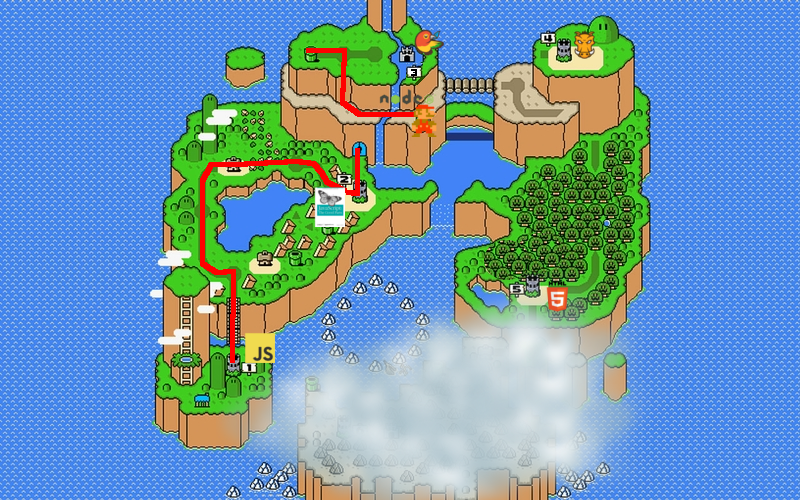
\includegraphics[width=300px]{images/map_bonus_stage_1.png}
  \end{center}
\end{frame}

\begin{frame}[fragile]
  \frametitle{What is Node.js?}
  \begin{block}{Website definition}
    Node.js is a platform built on Chrome's JavaScript runtime for easily building fast, scalable network applications. Node.js uses an event-driven, non-blocking I/O model that makes it lightweight and efficient, perfect for data-intensive real-time applications that run across distributed devices.
  \end{block}

  \begin{center}
    
\includegraphics[width=150px]{images/nodejs.png}
  \end{center}
\end{frame}

\begin{frame}[fragile]
  \frametitle{Installation}
  \begin{block}{From source-code or pre-built installer}
    Visit \url{http://nodejs.org/download/} and choose the package for your platform.
  \end{block}

  \pause

  \begin{block}{Using \texttt{nvm} (UNIX environments)}
    Visit \url{https://github.com/creationix/nvm} and follow instructions.
  \end{block}

  \pause

  \begin{block}{Check installation}
    {\scriptsize
    \begin{verbatim}
    $ node -v
    v0.8.21
    $ npm -v
    1.2.11
    \end{verbatim}
    }
  \end{block}
\end{frame}

\begin{frame}[fragile]
  \frametitle{Node packages}

  Node.js has a lot of packages that can be installed using \texttt{npm}. 
  You can publish your own code as a node package and it will be available through \texttt{npm}.

  \pause

  \begin{block}{Installing packages}
  {\scriptsize
  \begin{verbatim}
  $ npm install <package_name>
  \end{verbatim}
  }
  \end{block}
\end{frame}
